%!TEX root = ../report.tex

\begin{document}
    \chapter{Metrics}
    An extensive review was conducted to find a suitable metric that overcomes limitations of Negative-Log-Likelihood(NLL) in capturing the quality of approximated posterior distribution. The following metrics were considered for analysis:
    \begin{itemize}
	\item Brier score
	\item Expected Calibration Error
	\item Maximum Calibration Error
	\item Bayesian Information Criterion
	\item Mutual Information
	\item Entropy
	\item Cross Entropy
	\item Kullback-Leibler Divergence
	\item Signal to Noise Ratio
    \end{itemize}
	Though some of them suit for measuring calibration, sharpness and uncertainty estimation quality in a classification setup, none of them apply to regression due to the continuous nature of the output space. Understanding and approaching Deep Neural Networks from the perspective of Information theory\cite{saxe2019on} may prove helpful in devising a suitable metric to measure the quality of uncertainty estimates in the regression setup.
	\chapter{Correlation matrices for OOD analysis}
	The following are Spearman's correlation coefficient matrices for MCDO\_ADF and DER methods, obtained by relating variables involved in the extended Out-Of-Distribution response analysis described in \ref{ood_extended}. Apart from the strong correlation value between darkness levels(darkness\_coefficient) and prediction error(abs\_deviation), values of Spearman's coefficient for other pairs of variables do not mean much as they do not have a monotonic relationship (as observed from \ref{fig_ood_extended}), which is an important criterion for analysing a problem using Spearman's correlation analysis.
	\begin{figure}[H]
	\begin{subfigure}[b]{0.5\textwidth}
	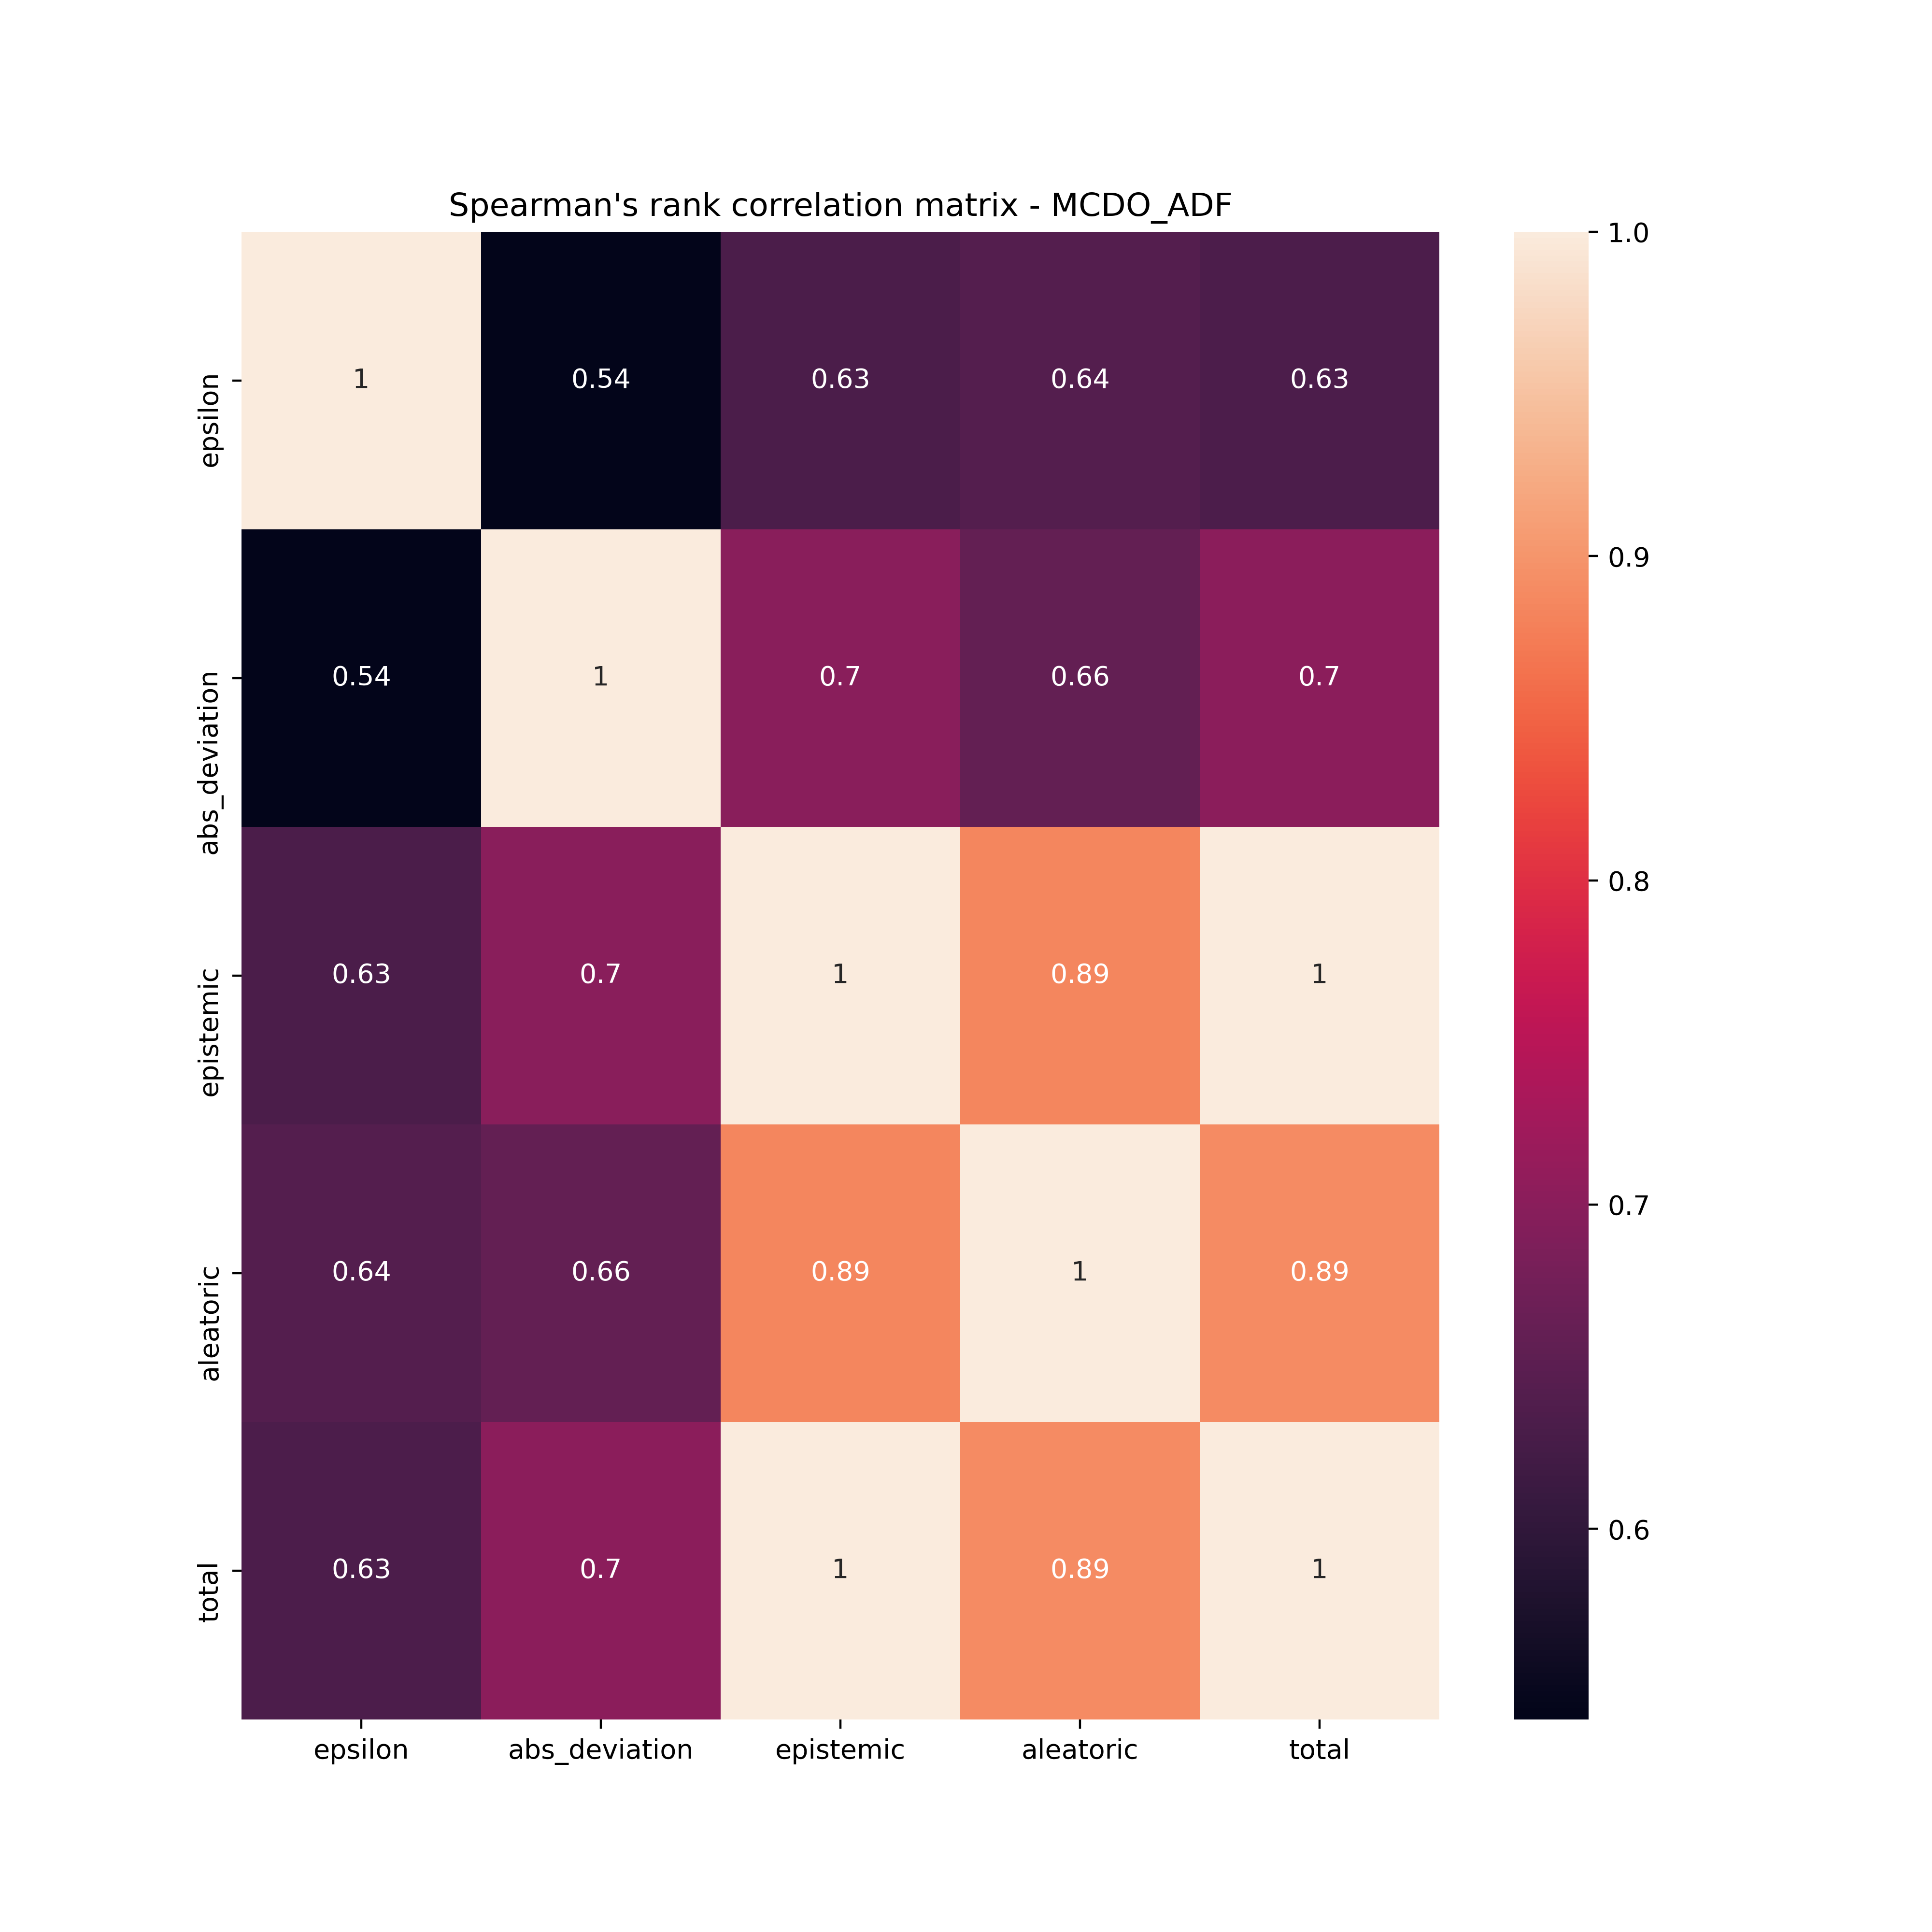
\includegraphics[width=1\textwidth,right]{ood/mcdo_adf_correlation_matrix}
	\caption{Spearman's correlation matrix-MCDO\_ADF}
	\label{homo_fn1}
	\end{subfigure}
	\hfill
	\begin{subfigure}[b]{0.5\textwidth}
	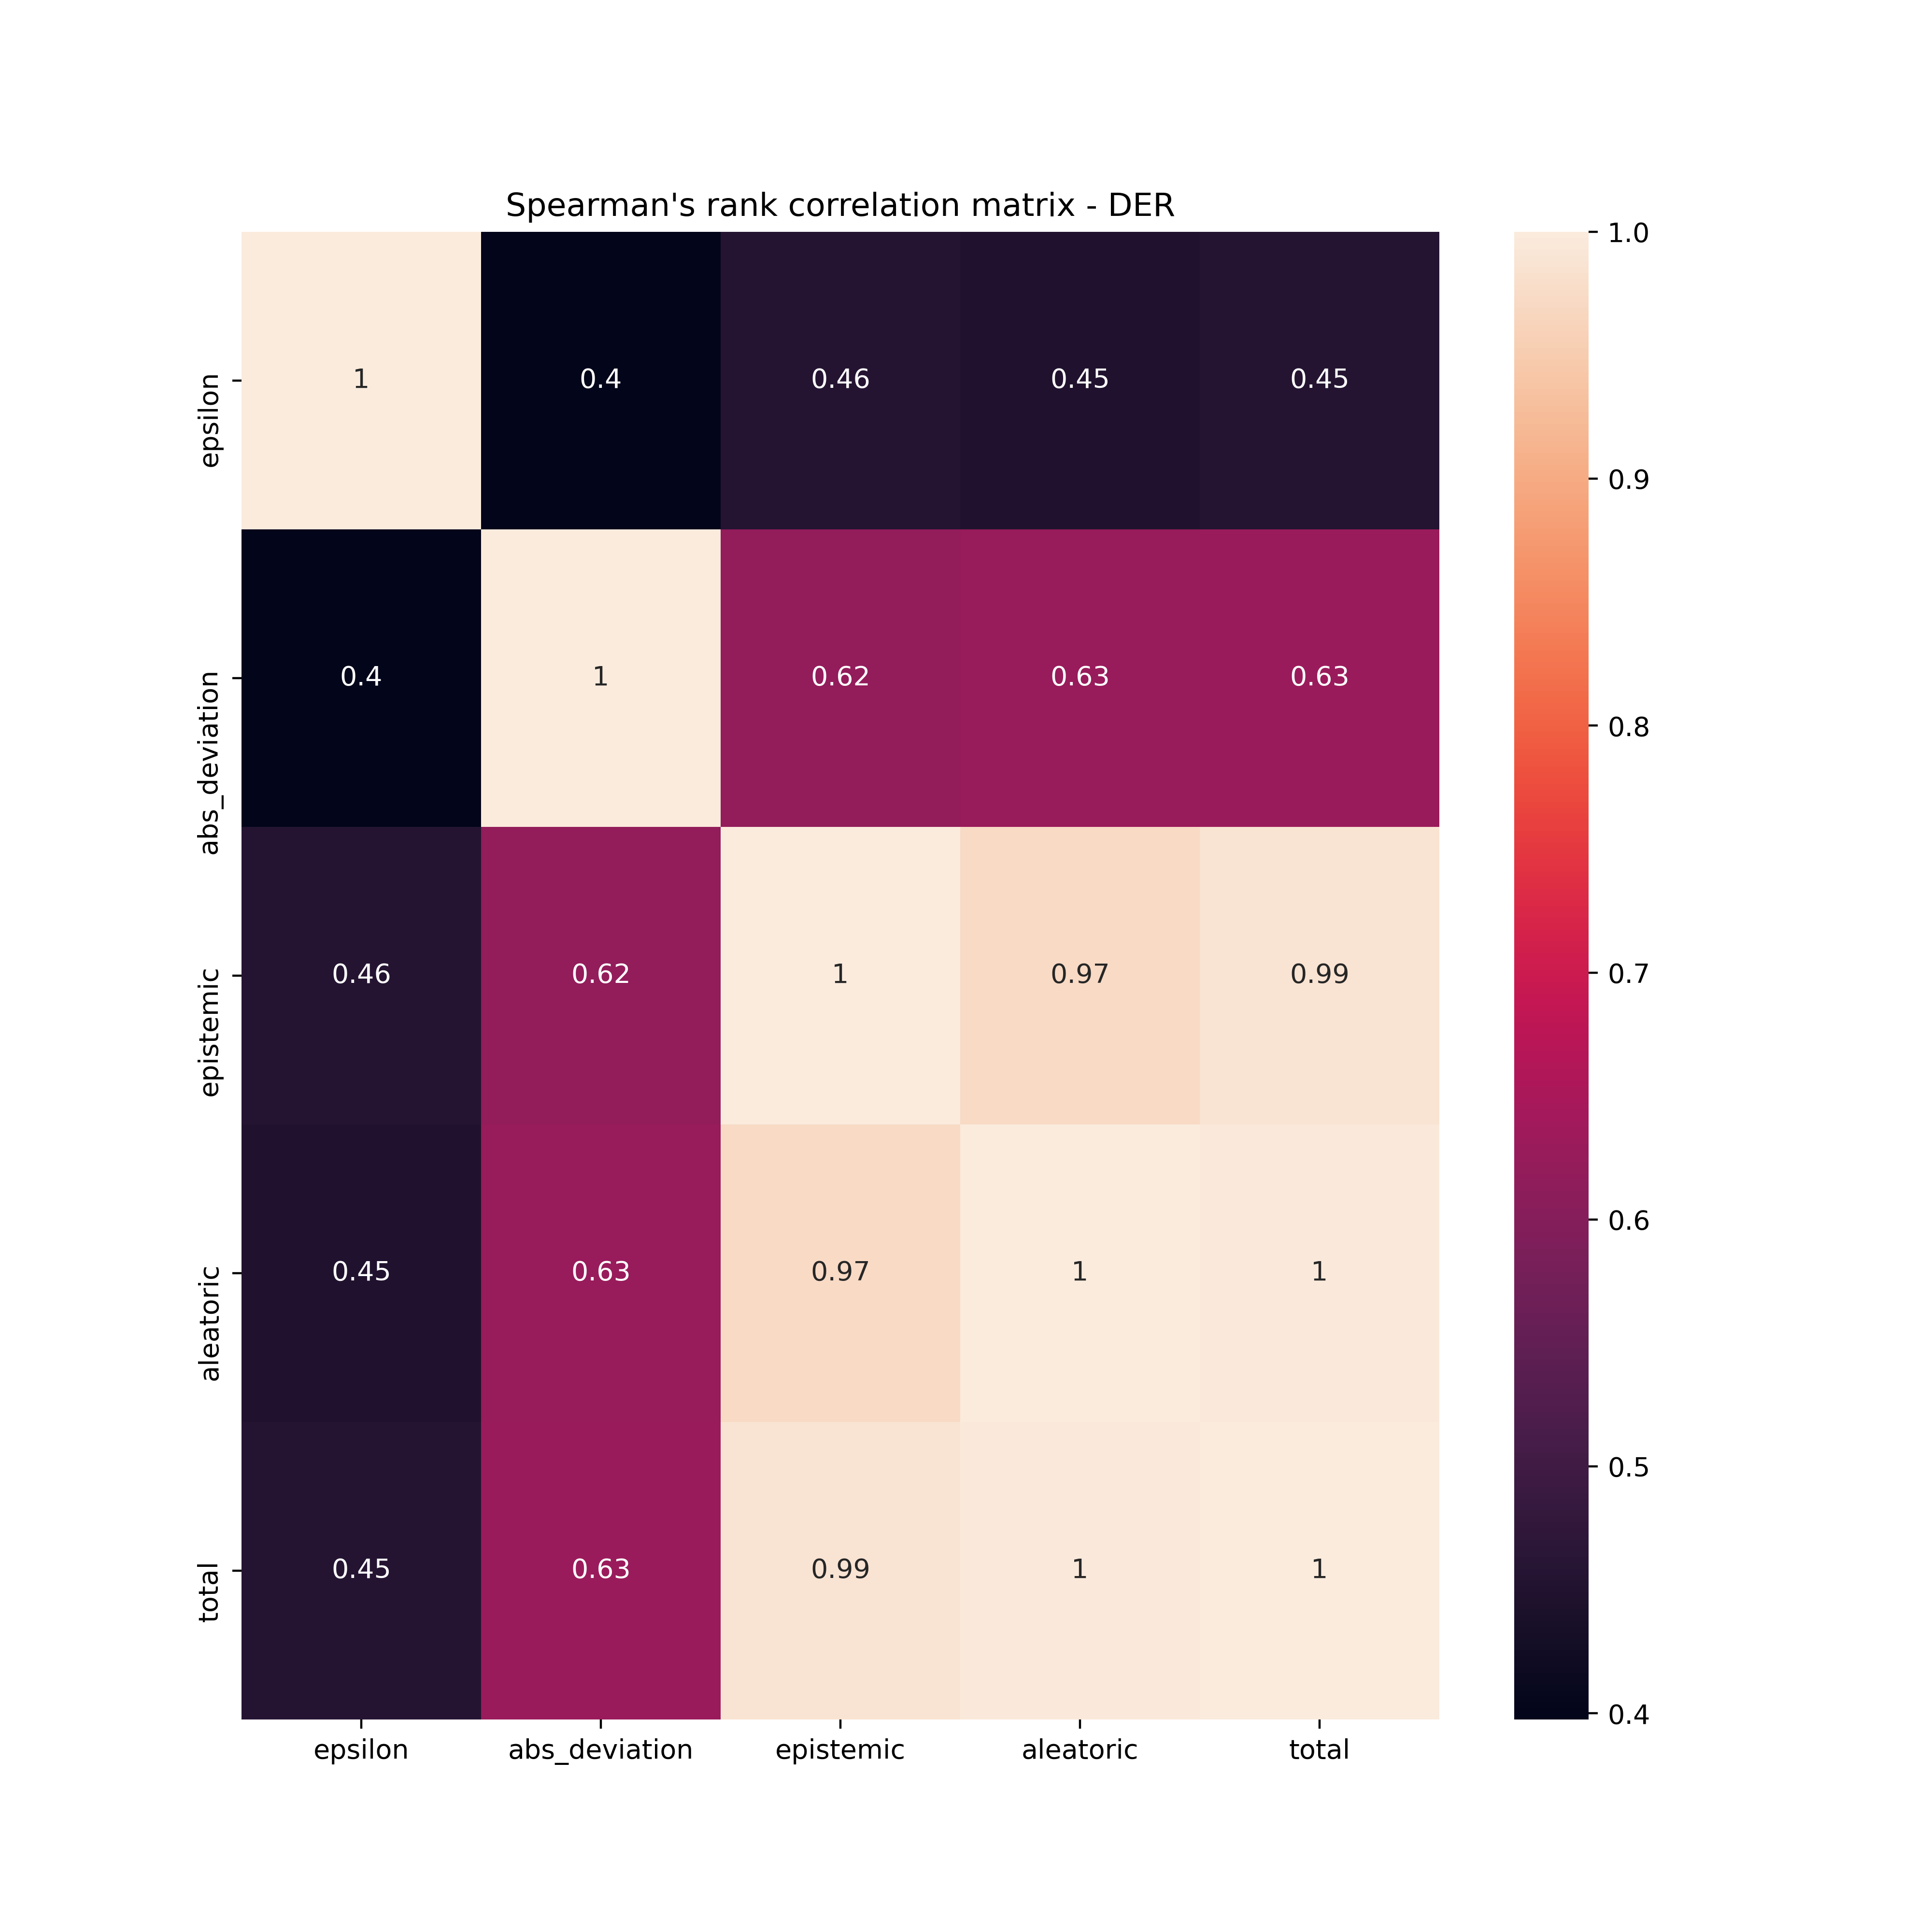
\includegraphics[width=1\textwidth,right]{ood/evi_correlation_matrix}
	\caption{Spearman's correlation matrix-DER}
	\label{hetero_fn1}
	\end{subfigure}
	\hfill
	\end{figure}
\end{document}
